\section{Where to paint}\label{sec:painting}

The whole stand is white. Colour only goes into the recessed lines, which act as masks: you flood the groove and wipe
the surface clean. Paint after the inserts are in and before the final assembly, part by part.

\begin{table}[H]
\centering
\caption{Painting map.}
\label{tab:paint}
\zebra
\begin{tabularx}{\linewidth}{@{}L{3.1cm}Y L{2.6cm}@{}}
\toprule
\thd{Part} & \thd{Feature} & \thd{Colour} \\
\midrule
01 Base           & Wrap-around light line, the groove halfway up the base & \paintblue \\
01 Base           & \code{@jmyounghoyos} engraving on the front & \paintblack\ or \paintred \\
04 Lower column   & Front channel (long recessed strip on the front facet) & \paintblue \\
04 Lower column   & Back channel & \paintred \\
04 Lower column   & Thin panel lines on both sides & \paintblack \\
05 Upper arm      & Front channel & \paintblue \\
05 Upper arm      & Back channel & \paintred \\
05 Upper arm      & Thin panel lines on both sides & \paintblack \\
06 VESA plate     & Four grooves along the X arms (back face) & \paintyellow \\
\bottomrule
\end{tabularx}
\end{table}

\begin{step}{Painting process}
\begin{enumerate}
  \item Clean the parts with isopropyl alcohol. Lightly sand the edges of the grooves with 400 grit if there is stringing.
  \item \textbf{Channels and the light line:} use an extra-fine paint marker (Posca PC-1MR or PC-3M) or acrylic with a 0/00
        brush. Flood the groove, then wipe the surface right away with a cloth barely damp with water or alcohol.
  \item \textbf{Panel lines and engraving:} thin black acrylic about 1:3 with water and a drop of dish soap, run it along the
        line so capillarity pulls it in, and wipe the excess after a minute.
  \item Optional: one coat of water-based matte varnish to protect the paint from hands.
\end{enumerate}
\end{step}

\begin{figure}[H]
  \centering
  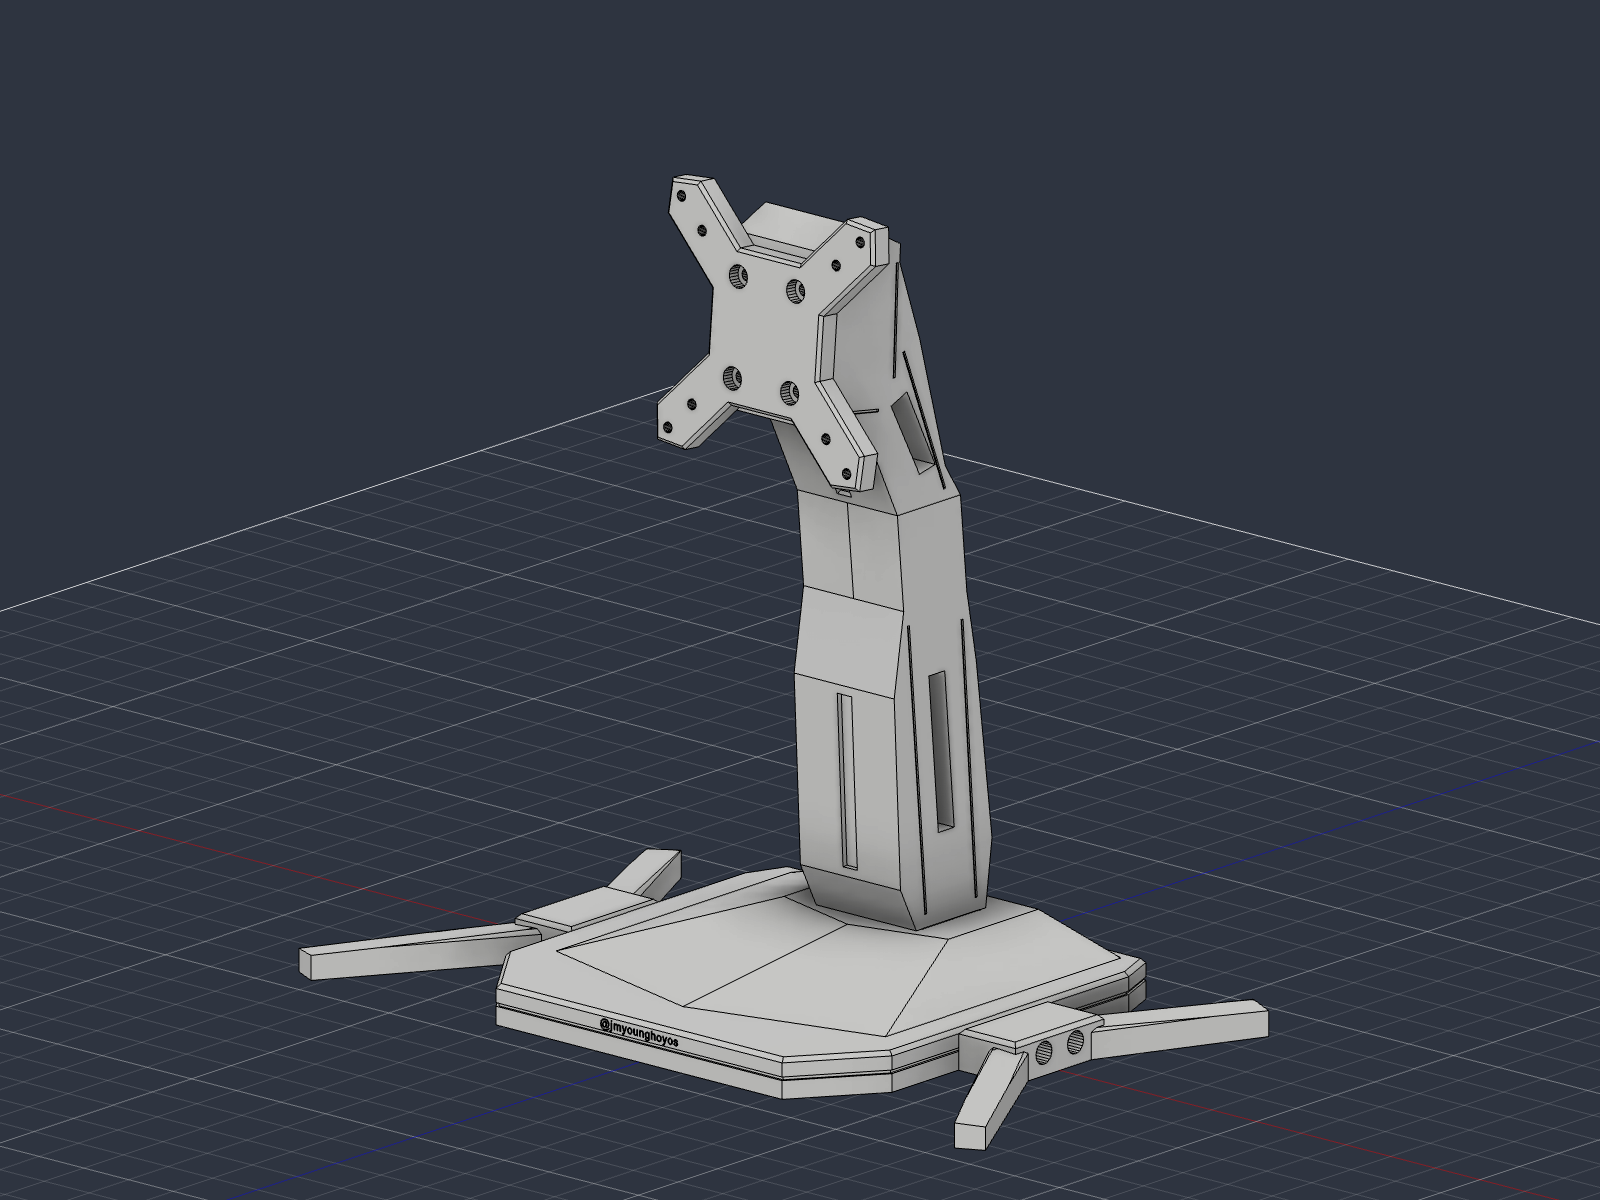
\includegraphics[width = 0.42\linewidth]{assembly-front.png}
  \caption{Front view. The light line runs around the base; the column and arm channels face front and back.}
\end{figure}
